\documentclass[../../main.tex]{subfiles}
\graphicspath{{../../image/}{../../figure/}}
\begin{document}

\section{特征族真正非线性或线性退化的方程组}\label{section:ch09-真正非线性或线性退化方程组}

我们在此的目标是为波特别简单的方程组构造波曲线。当第 $i$ 特征族线性退化时,不存在中心 $i$-稀疏波,因而由\cref{theorem:ch08-重合条件},任一 $i$-波必为 $i$-接触间断。此时前向与后向 $i$-波曲线重合于\cref{theorem:ch08-重合条件}中的激波曲线 $W_{i}$,即
\begin{align}
\Phi_{i}(\tau;\bar{U})=\Psi_{i}(\tau;\bar{U})=W_{i}(\tau;\bar{U}).\nonumber
\end{align}

当第 $i$ 特征族真正非线性时, $i$-接触间断被\cref{theorem:ch07-稀疏波曲线存在唯一}排除,因而任一微小振幅 $i$-波必为单个中心 $i$-稀疏波或单个压缩 $i$-激波。将场 $R_{i}$ 规范化使\cref{theorem:ch07-稀疏波曲线存在唯一}成立,即 $\mathrm{D}\lambda_{i}R_{i}=1$。可由弱 $i$-激波连接到 $\bar{U}$ 的状态位于\cref{theorem:ch07-稀疏波曲线存在唯一}所述的 $i$-激波曲线 $W_{i}(\tau;\bar{U})$ 上。由\cref{theorem:ch07-稀疏波曲线存在唯一},从左侧连接 $\bar{U}$ 到右侧 $W_{i}(\tau;\bar{U})$ 的激波为压缩激波当且仅当 $\tau<0$。另一方面,由\cref{theorem:ch07-稀疏波曲线存在唯一},状态 $\bar{U}$ 的右侧(或左侧)可由中心 $i$-稀疏波连接到状态 $V_{i}(\tau;\bar{U})$,其中 $\tau>0$(或 $\tau<0$)。于是可这样构造前向 $i$-波曲线: $\tau<0$ 时 $\Phi_{i}(\tau;\bar{U})=W_{i}(\tau;\bar{U})$, $\tau>0$ 时 $\Phi_{i}(\tau;\bar{U})=V_{i}(\tau;\bar{U})$。类似地,后向 $i$-波曲线定义为: $\tau<0$ 时 $\Psi_{i}(\tau;\bar{U})=V_{i}(\tau;\bar{U})$, $\tau>0$ 时 $\Psi_{i}(\tau;\bar{U})=W_{i}(\tau;\bar{U})$。由\cref{theorem:ch07-稀疏波曲线存在唯一},这些曲线是 $C^{2,1}$ 的;并由\cref{theorem:ch07-稀疏波曲线存在唯一}满足\eqref{align:ch09-9-3-2}、\eqref{align:ch09-9-3-3}与\eqref{align:ch09-9-3-7}。

基于上述讨论,我们现已对特征族要么真正非线性、要么线性退化的方程组建立了 Riemann 问题解的存在性:

\begin{theorem}\label{theorem:ch09-小振幅riemann解}
假定方程组\eqref{align:ch09-9-1-1}严格双曲,且每个特征族要么真正非线性、要么线性退化。当 $|U_{R}-U_{L}|$ 充分小时, Riemann 问题\eqref{align:ch09-9-1-1}、\eqref{align:ch09-9-1-18}存在唯一的自相似解\eqref{align:ch09-9-1-2},其全变差小。该解由 $n+1$ 个常值状态 $U_{L}=U_{0},U_{1},\dots,U_{n-1},U_{n}=U_{R}$ 组成。当第 $i$ 特征族线性退化时, $U_{i}$ 与 $U_{i-1}$ 由 $i$-接触间断连接;当第 $i$ 特征族真正非线性时, $U_{i}$ 与 $U_{i-1}$ 由一个中心 $i$-稀疏波或一个压缩 $i$-激波连接。
\end{theorem}

特别地,\cref{theorem:ch09-小振幅riemann解}适用于等熵气体动力学方程组\eqref{align:ch07-等熵Euler}的 Riemann 问题,条件是 $2p'(\rho)+\rho p''(\rho)>0$,此时两个特征族都真正非线性;也适用于绝热热弹性方程组\eqref{align:ch07-热弹性},条件是 $p_{uu}(u,s)\neq0$,此时第 $1$、第 $3$ 特征族真正非线性,而第 $2$ 特征族线性退化。

作为简单示例,考虑 Lagrange 坐标下等熵热弹性方程组\eqref{align:ch07-p系统},假定 $\sigma(u)$ 定义在 $(-\infty,\infty)$ 上,且 $0<a\leqslant\sigma'(u)\leqslant b<\infty$, $\sigma''(u)<0$。在此条件下,波曲线整体有定义,即使端状态 $(u_{L},v_{L})$ 与 $(u_{R},v_{R})$ 相距甚远,Riemann 问题也可求解。方便起见,取 $u$ 为新参数重新参数化波曲线。此时,过状态空间典型点 $(\bar{u},\bar{v})$ 的前向 $1$-波曲线 $\Phi_{1}$ 与后向 $2$-波曲线 $\Psi_{2}$ 可分别表示为 $v=\varphi(u;\bar{u},\bar{v})$ 与 $v=\psi(u;\bar{u},\bar{v})$。回顾此方程组 Hugoniot 轨迹\eqref{align:ch08-rdr}与稀疏波曲线\eqref{align:ch07-p系统稀疏波}的形式,我们推得
\begin{align}
\varphi(u;\bar{u},\bar{v})=
\begin{cases}
\bar{v}-\sqrt{[\sigma(u)-\sigma(\bar{u})](u-\bar{u})},&u\leqslant\bar{u},\\
\bar{v}+\displaystyle\int_{\bar{u}}^{u}\sqrt{\sigma'(\omega)}\,\mathrm{d}\omega,&u>\bar{u},
\end{cases}
\label{align:ch09-9-4-1}
\end{align}
\begin{align}
\psi(u;\bar{u},\bar{v})=
\begin{cases}
\bar{v}+\sqrt{[\sigma(u)-\sigma(\bar{u})](u-\bar{u})},&u\leqslant\bar{u},\\
\bar{v}-\displaystyle\int_{\bar{u}}^{u}\sqrt{\sigma'(\omega)}\,\mathrm{d}\omega,&u>\bar{u}.
\end{cases}
\label{align:ch09-9-4-2}
\end{align}

\cref{figure:ch09-压缩激波与稀疏波}描绘了一个 Riemann 问题的解,它由一个压缩 $1$-激波与一个中心 $2$-稀疏波组成。中间常值状态 $(u_{M},v_{M})$ 在 $u$-$v$ 平面上确定为过 $(u_{L},v_{L})$ 的前向 $1$-波曲线 $\Phi_{1}$ 与过 $(u_{R},v_{R})$ 的后向 $2$-波曲线 $\Psi_{2}$ 的交点,即求解方程
\begin{align}
v_{M}=\varphi(u_{M};u_{L},v_{L})=\psi(u_{M};u_{R},v_{R}).
\label{align:ch09-9-4-3}
\end{align}

\begin{figure}[ht]
\centering
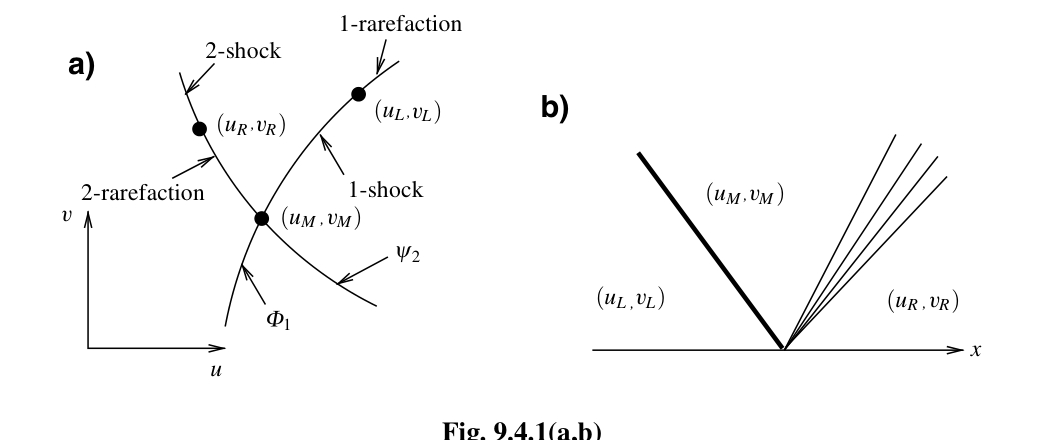
\includegraphics[width=0.85\textwidth]{ch09-fig04-01.png}
\caption{(a) $u$-$v$ 平面上的前向 $1$-波曲线 $\Phi_{1}$ 与后向 $2$-波曲线 $\Psi_{2}$;中间状态 $(u_{M},v_{M})$ 为交点。(b) 相应的 $x$-$t$ 平面波扇。}
\label{figure:ch09-压缩激波与稀疏波}
\end{figure}

对两个守恒律的方程组,在 Riemann 不变量平面上而非原状态空间中构造中间常值状态往往是方便的。原因是,如\cref{section:ch07-简单波}所指出,在 Riemann 不变量平面上稀疏波曲线成为平行于坐标轴的直线。这大大便利了定位不同特征族波曲线交点的工作。\cref{figure:ch09-riemann不变量平面}描绘了\cref{figure:ch09-压缩激波与稀疏波}中波曲线在 Riemann 不变量 $w$-$z$ 平面上的构型。

\begin{figure}[ht]
\centering
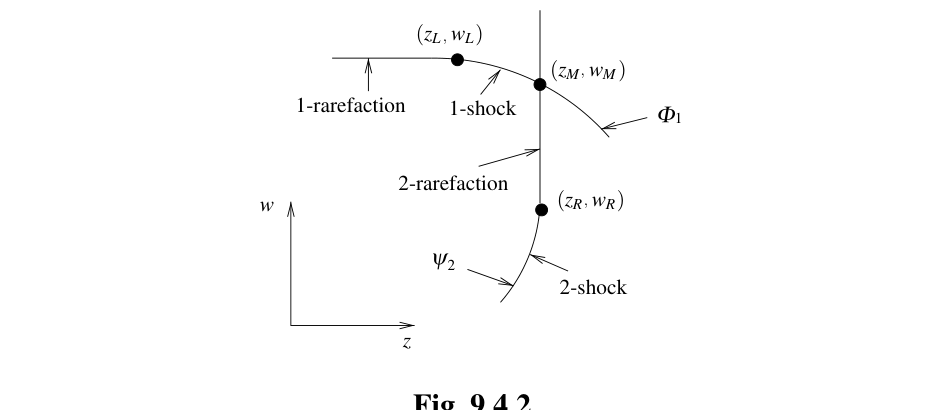
\includegraphics[width=0.7\textwidth]{ch09-fig04-02.png}
\caption{\cref{figure:ch09-压缩激波与稀疏波}的波曲线在 Riemann 不变量 $w$-$z$ 平面上的构型:稀疏波曲线为平行于坐标轴的直线。}
\label{figure:ch09-riemann不变量平面}
\end{figure}

特别地,端状态为 $(u_{L},v_{L})$、解如上述由压缩 $1$-激波与 $2$-稀疏波组成的 Riemann 问题,是由一个压缩 $1$-激波(连接状态 $(u_{L},v_{L})$ 与 $(u_{0},v_{0})$)与一个较慢的压缩 $1$-激波(连接 $(u_{0},v_{0})$ 与 $(u_{R},v_{R})$)碰撞所产生的。类似地,两个压缩 $2$-激波的碰撞导致的 Riemann 问题,其解由一个 $1$-稀疏波与一个压缩 $2$-激波组成。

当\eqref{align:ch07-p系统}中的介质是气体时,情况更复杂,此时当 $u\to\infty$ 时 $\sigma'(u)\to0$。这将在\cref{section:ch09-存在性与唯一性的失效}中讨论。

Riemann 问题最著名的例子,是关于支配无粘气体在管道中绝热直线流动的质量、动量与能量守恒律方程组。该问题的详尽处理可见\cref{section:ch09-注记}所引文献,故此处简要介绍即可。该问题通常在方程组的 Euler 形式下考虑,即\eqref{align:ch03-Euler}的一维版本,以密度 $\rho$、速度 $v$、压力 $p$ 为状态变量,激波曲线以 $p$ 参数化。然而这里我们处理 Lagrange 形式\eqref{align:ch07-热弹性},状态变量为比容 $u$、速度 $v$ 与熵 $s$。此外,激波曲线以 $u$ 参数化。这种做法便于借助把 $s(u)$ 表示为微分方程\eqref{align:ch08-riemann恒等式}解的表示,将激波曲线延拓到强激波领域。

我们假定 $p_{u}<0$(双曲性所需), $p_{uu}>0$,从而第 $1$、第 $3$ 特征族真正非线性;并假定 $p_{s}=-\theta_{u}>0$,从而使 $1$-与 $3$-激波曲线的微分方程\eqref{align:ch08-riemann恒等式}大范围适定。第 $2$ 特征族线性退化。

在上述假设下,端状态为 $(u_{L},v_{L},s_{L})$ 与 $(u_{R},v_{R},s_{R})$ 的 Riemann 问题的解,预期由一个压缩 $1$-激波或 $1$-稀疏波(连接 $(u_{L},v_{L},s_{L})$ 与某状态 $(u_{M}^{-},v_{M}^{-},s_{M}^{-})$),继之以一个静止接触间断(连接 $(u_{M}^{-},v_{M}^{-},s_{M}^{-})$ 与某状态 $(u_{M}^{+},v_{M}^{+},s_{M}^{+})$),再继之以一个压缩 $3$-激波或 $3$-稀疏波(连接 $(u_{M}^{+},v_{M}^{+},s_{M}^{+})$ 与 $(u_{R},v_{R},s_{R})$)组成。上述状态对应的压力记为 $p_{L},p_{M}^{-},p_{M}^{+},p_{R}$。接触间断的 Rankine-Hugoniot 跳跃条件要求 $v_{M}^{-}=v_{M}^{+}=v_{M}$ 且 $p_{M}^{-}=p_{M}^{+}=p_{M}$。因而,为求解 Riemann 问题,跟踪波曲线在 $v$-$p$ 平面上的投影是方便的。

$1$-与 $3$-激波曲线由\eqref{align:ch08-riemann恒等式}、\eqref{align:ch08-rh曲线}确定,而 $1$-与 $3$-稀疏波曲线由\eqref{align:ch07-热弹性稀疏波}给出。因此,过状态 $(\bar{u},\bar{v},\bar{s})$、以 $u$ 参数化的前向 $1$-波曲线与后向 $3$-波曲线的投影 $\Phi$、$\Psi$ 为
\begin{align}
\Phi(u;\bar{u},\bar{v},\bar{s})=
\begin{cases}
\bigl(\bar{v}-\sqrt{[-p(u,s(u))+p(\bar{u},\bar{s})](u-\bar{u)}},\ p(u,s(u))\bigr),&u\leqslant\bar{u},\\
\bigl(\bar{v}+\displaystyle\int_{\bar{u}}^{u}\sqrt{-p_{\omega}(\omega,\bar{s})}\,\mathrm{d}\omega,\ p(u,\bar{s})\bigr),&u>\bar{u},
\end{cases}
\label{align:ch09-9-4-4}
\end{align}
\begin{align}
\Psi(u;\bar{u},\bar{v},\bar{s})=
\begin{cases}
\bigl(\bar{v}+\sqrt{[-p(u,s(u))+p(\bar{u},\bar{s})](u-\bar{u)}},\ p(u,s(u))\bigr),&u\leqslant\bar{u},\\
\bigl(\bar{v}-\displaystyle\int_{\bar{u}}^{u}\sqrt{-p_{\omega}(\omega,\bar{s})}\,\mathrm{d}\omega,\ p(u,\bar{s})\bigr),&u>\bar{u},
\end{cases}
\label{align:ch09-9-4-5}
\end{align}
其中 $s(u)$ 表示\eqref{align:ch08-riemann恒等式}满足初值 $s(\bar{u})=\bar{s}$ 的解。Riemann 问题的解由曲线 $\Phi(\cdot;u_{L},v_{L},s_{L})$ 与 $\Psi(\cdot;u_{R},v_{R},s_{R})$ 的交点生成:
\begin{align}
(v_{M},p_{M})=\Phi(u_{M}^{-};u_{L},v_{L},s_{L})=\Psi(u_{M}^{+};u_{R},v_{R},s_{R}).
\label{align:ch09-9-4-6}
\end{align}

正如\cref{theorem:ch09-小振幅riemann解}所断言,当 $(u_{L},v_{L},s_{L})$ 与 $(u_{R},v_{R},s_{R})$ 彼此接近时,存在唯一局部交点,从而存在 Riemann 问题的唯一解。$1$-与 $3$-波是压缩激波还是稀疏波,取决于端状态在状态空间中的相对位置。我们不拟在此对可能的波构型作完全分类,因为这可在\cref{section:ch09-注记}所引文献中找到。作为说明性例子,考虑理想气体\eqref{align:ch02-2-5-20}、$\gamma\leqslant5/3$ 时第三族两个压缩激波碰撞诱导的 Riemann 问题,其解由第三族一个压缩激波、第一族一个稀疏波与一个接触间断组成,如\cref{figure:ch09-气体激波碰撞}所示。与之相对,当 $\gamma>5/3$ 时,同族两个弱压缩激波的碰撞产生两族压缩激波连同一个接触间断。

波曲线 $\Phi$ 与 $\Psi$ 是整体定义的,因而与等熵情形一样,即使端状态相距甚远也可用它们求解 Riemann 问题。对此问题的研究表明:取决于状态方程以及 $(u_{L},v_{L},s_{L})$ 与 $(u_{R},v_{R},s_{R})$ 的相对位置,这两条波曲线可能交于一点、交于多点,或根本不相交,相应地给出 Riemann 问题的唯一解、多个解或无解。

\begin{figure}[ht]
\centering
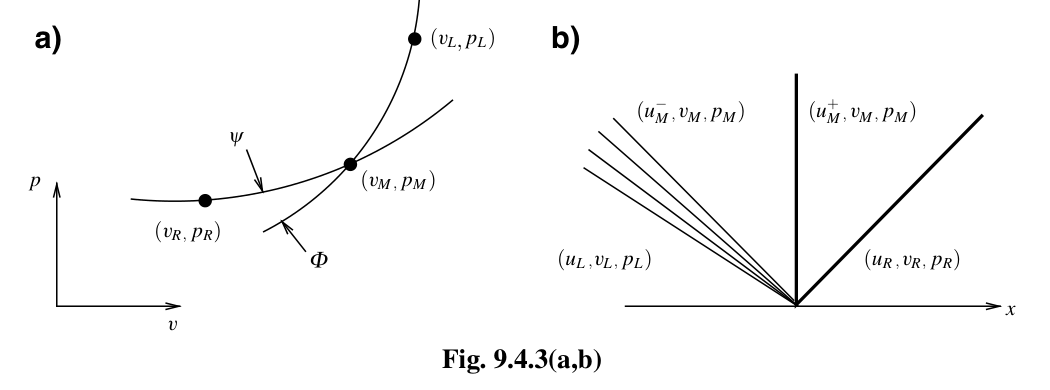
\includegraphics[width=0.85\textwidth]{ch09-fig04-03.png}
\caption{(a) $v$-$p$ 平面上前向 $1$-波曲线投影 $\Phi$ 与后向 $3$-波曲线投影 $\Psi$ 的交点;接触间断两侧为 $(u_{M}^{-},v_{M},p_{M})$ 与 $(u_{M}^{+},v_{M},p_{M})$。(b) 相应的 $x$-$t$ 平面波扇。}
\label{figure:ch09-气体激波碰撞}
\end{figure}

\end{document}
